 
\chapter{工具变量方法的应用：孟德尔随机化}
 \label{chapter::iv-mr}




\citet{katan1986apoupoprotein}研究了某些观察性研究的结果，这些研究表明低血清胆固醇水平与癌症风险相关。然而，正如我们所讨论的，观察性研究容易受到未测量混杂因素的影响。因此，很难将观察到的关联性解释为因果关系。在\citet{katan1986apoupoprotein}所研究的具体问题中，甚至有可能是癌症的早期阶段导致了血清胆固醇水平降低。利用常规的流行病学研究方法，要厘清血清胆固醇水平对癌症的因果效应似乎是个难题。\citet{katan1986apoupoprotein}指出，载脂蛋白E基因与血清胆固醇水平相关，但并不直接影响癌症的发生。因此，如果低血清胆固醇水平确实会导致癌症，那么在具有该基因型的人群与不具备该基因型的人群之间，其癌症风险应当存在显著差异。用因果推断的术语来说，\citet{katan1986apoupoprotein}提出将载脂蛋白E基因作为工具变量来使用。 


\citet{katan1986apoupoprotein}并未开展数据分析，只是提出了一种概念性设计，以同时应对{\it 未测量混杂}和{\it 反向因果}。此后，得益于现代全基因组关联研究，人们开展了更复杂精细的研究。这些研究将遗传信息作为流行病学研究中暴露的工具变量，估计暴露对结果的因果效应。其思想均源于{\it 孟德尔第二定律}，即{\it 自由组合定律}，它指出一种性状的遗传独立于其他性状的遗传。因此，使用遗传信息作为工具变量的方法称为{\it 孟德尔随机化}（MR）。 


\section{背景与动机}

从图表上看，图\ref{fig::mr-dag}呈现了处理因素$D$、结局变量$Y$、未测量混杂因素$U$以及遗传工具变量$G_1, \ldots, G_p$之间的因果关系。在多数MR研究中，这些遗传工具变量往往是单核苷酸多态性位点（SNP）。由于多效性现象的存在\footnote{多效性是指一个基因可同时影响两个或多个看似无关的表型特征}，这些遗传工具变量也可能直接影响目标结局。因此，图\ref{fig::mr-dag}也考虑了排除性假设可能被违反的情形。  

\begin{figure}
\centering
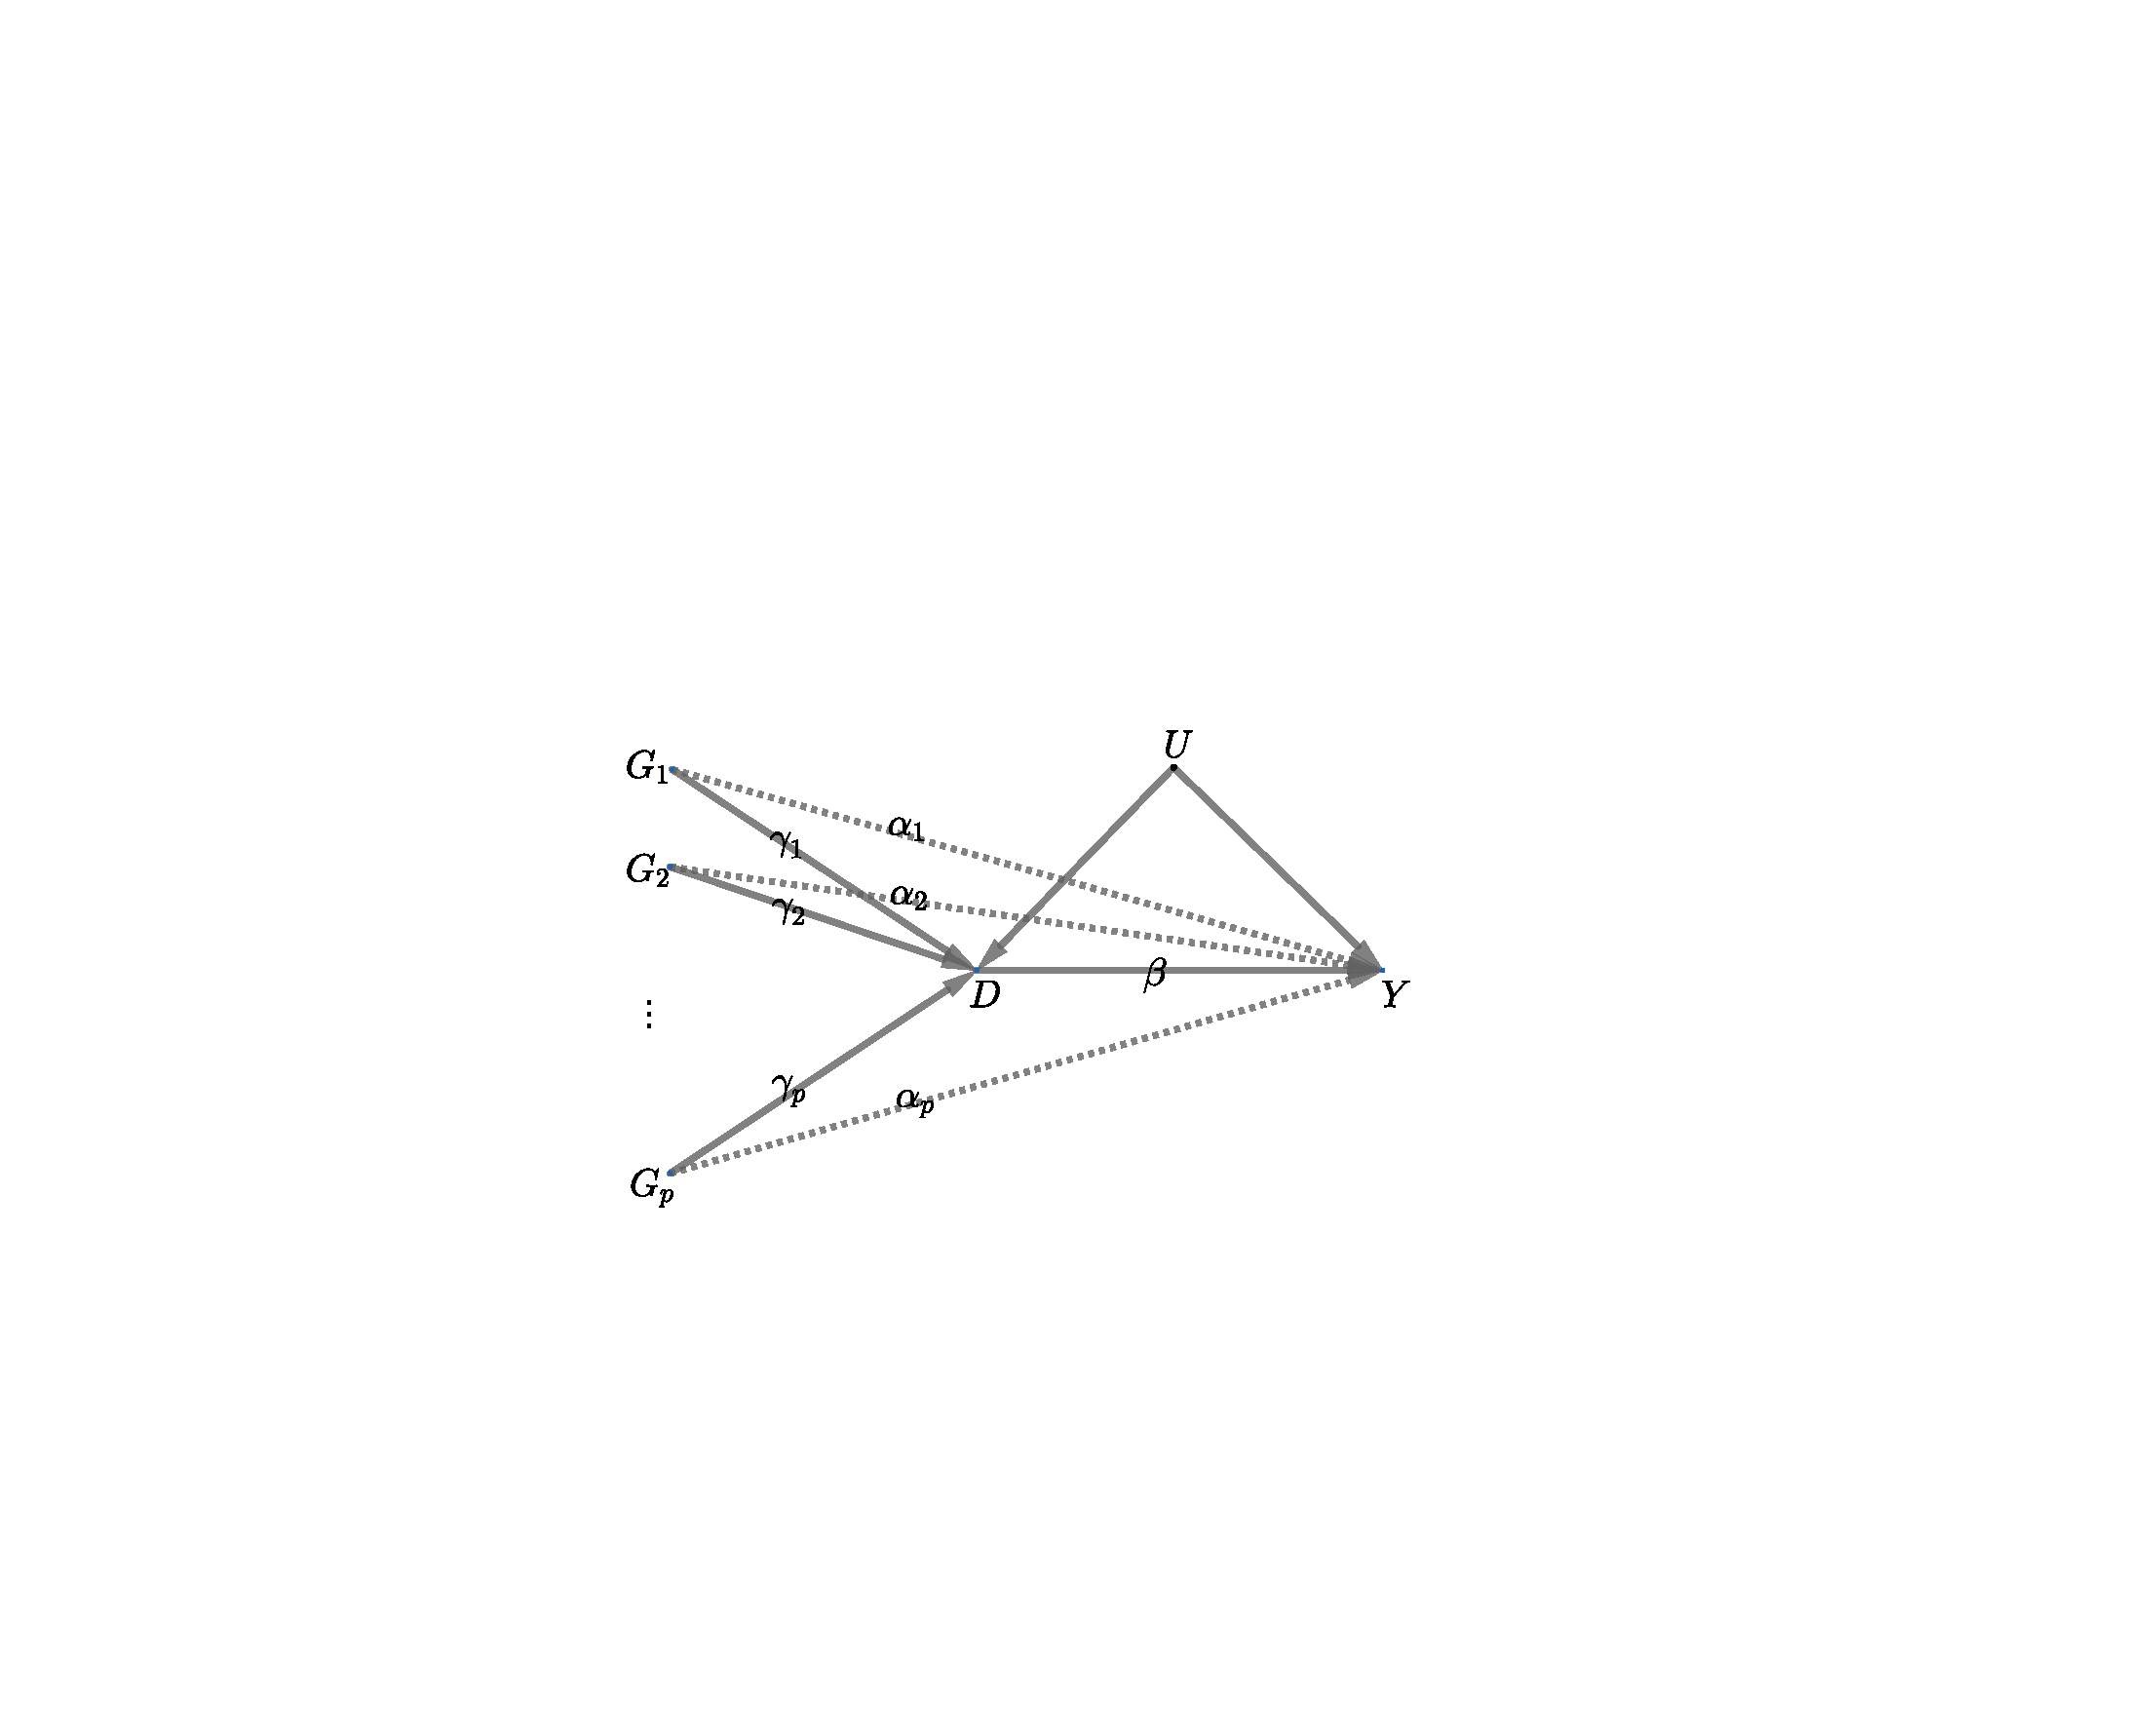
\includegraphics[width = 0.8 \textwidth]{figures/mr_dag.pdf}
\caption{孟德尔随机化的因果图}\label{fig::mr-dag}
\end{figure}



标准的线性工具变量模型通常假设工具变量对结局无直接效应。下面的定义\ref{def::linear-iv-model-mr}分别给出了该模型的结构形式及简化形式。 

\begin{definition}
[线性工具变量模型]\label{def::linear-iv-model-mr}
标准线性工具变量模型\begin{eqnarray}
Y  &=& \beta_0 +  \beta D + \beta_u U + \varepsilon_Y , \\
D  &=& \gamma_0 +   \gamma_1 G_1 + \cdots + \gamma_p G_p + \gamma_u U + \varepsilon_D ,
\end{eqnarray}的简约式为\begin{eqnarray}
Y  &=&\beta_0 +  \beta  \gamma_0 + \beta \gamma_1 G_1 + \cdots + \beta  \gamma_p G_p  + (\beta_u + \beta_0 \gamma_u )U + \varepsilon_Y , \\
D  &=& \gamma_0 +  \gamma_1 G_1 + \cdots + \gamma_p G_p + \gamma_u U + \varepsilon_D ,
\end{eqnarray}
\end{definition}



定义\ref{def::linear-model-invalid-iv-mr}则允许排除性假设被违反的情况；在此情形下，$G_1, \ldots, G_p$便不再符合有效工具变量的条件。 


\begin{definition}
[可能存在无效工具变量的线性模型]\label{def::linear-model-invalid-iv-mr}
线性模型\begin{eqnarray}
Y  &=& \beta_0 + \beta D + \alpha_1 G_1 + \cdots + \alpha_p G_p  + \beta_u U + \varepsilon_Y ,   \\
D  &=& \gamma_0 + \gamma_1 G_1 + \cdots + \gamma_p G_p + \gamma_u U + \varepsilon_D ,
\end{eqnarray}的简约式为\begin{eqnarray}
Y  &=& ( \beta_0 +\beta  \gamma_0 ) +  (\alpha_1 + \beta \gamma_1)  G_1 + \cdots + (\alpha_p +  \beta  \gamma_p) G_p \nonumber  \\
&&+  ( \beta_u + \beta \gamma_u )  U + \varepsilon_Y ,   \\
D  &=& \gamma_0 +  \gamma_1 G_1 + \cdots + \gamma_p G_p + \gamma_u U + \varepsilon_D .
\end{eqnarray}
\end{definition}

定义\ref{def::linear-iv-model-mr}与\ref{def::linear-model-invalid-iv-mr}与第\ref{chapter::iv-econometric}章中介绍的线性工具变量模型略有差异，它们显式地引入了混杂因素$U$；不过这一细微差别并未从本质上改变讨论框架。 


在符合排除性假设的定义\ref{def::linear-iv-model-mr}中，我们有：
$$
\Gamma_j = \beta \gamma_j,\quad (j=1,\ldots,p).
$$
而在排除性假设被违反时，即定义\ref{def::linear-model-invalid-iv-mr}中，则有：
$$
\Gamma_j = \alpha_j +   \beta \gamma_j,\quad (j=1,\ldots,p). 
$$



若有个体数据，可在定义\ref{def::linear-iv-model-mr}中的线性工具变量模型下，用经典两阶段最小二乘估计量估计$\beta$。然而，大多数MR研究只有来自多个全基因组关联研究的汇总统计量，没有个体数据。典型的汇总统计量MR研究具有以下数据结构。


\begin{assumption}
[基于汇总统计量的孟德尔随机化研究]\label{assume::MR-summary}
(a)
我们可获得处理因素与遗传工具变量之间的回归系数$\hat{\gamma}_1   , \ldots, \hat{\gamma}_p$，以及对应的标准误$\se_{D1}, \ldots, \se_{Dp}$。假设：
\begin{eqnarray}
\label{eq::small-gammas}
\hat{\gamma}_1  \rightarrow \gamma_1 , \ldots, \hat{\gamma}_p \rightarrow \gamma_p
\end{eqnarray}
在概率意义上成立，且忽略标准误的不确定性。 

(b) 已知结果对遗传工具变量的回归系数$\hat{\Gamma}_1   , \ldots, \hat{\Gamma}_p$及其标准误$\se_{Y1}, \ldots, \se_{Yp}.$。假设\begin{eqnarray}
\label{eq::big-gammas}
\hat{\Gamma}_1 \rightarrow \Gamma_1 , \ldots, \hat{\Gamma}_p \rightarrow \Gamma_p
\end{eqnarray}依概率成立，并忽略标准误中的不确定性。  

(c)
假设$\hat{\gamma}_1   , \ldots, \hat{\gamma}_p, \hat{\Gamma}_1   , \ldots, \hat{\Gamma}_p$均为联合正态分布且彼此独立。
\end{assumption}


%\begin{eqnarray}
%\label{eq::small-gammas}
%\hat{\gamma}_1  \rightarrow \gamma_1 , \ldots, \hat{\gamma}_p \rightarrow \gamma_p
%\end{eqnarray}
%in probability with standard errors
%\begin{eqnarray}
%\label{eq::small-gammas-se}
%\se_{D1}, \ldots, \se_{Dp},
%\end{eqnarray}
%and the regression coefficients of the outcome on  the  genetic IVs:
%\begin{eqnarray}
%\label{eq::big-gammas}
%\hat{\Gamma}_1 \rightarrow \Gamma_1 , \ldots, \hat{\Gamma}_p \rightarrow \Gamma_p
%\end{eqnarray}
%in probability with standard errors
%\begin{eqnarray}
%\label{eq::big-gammas-se}
%\se_{Y1}, \ldots, \se_{Yp}.
%\end{eqnarray}

回归系数的渐近正态性可以由中心极限定理说明。在大样本中，标准误估计准确地估计真实标准误。因此，唯一较微妙的假设是各回归系数联合独立。$\hat{\gamma}_j$与$\hat{\Gamma}_j$之间的独立性是合理的，因为它们通常基于不同样本计算。 

若各$G_j$独立，且$D$的真实线性模型具有同方差误差项，则各$\hat{\gamma}_j$之间的独立性可能合理，见第\ref{section::linear-model-var}章。但当线性模型误差项存在异方差时，这个假设就变得微妙。若各$G_j$不独立，就很难说明估计量相互独立。若回归系数来自非线性模型，则更难说明这种独立性。各$\hat{\Gamma}_j$之间的独立性可作类似讨论。 

本章重点讨论如何根据假设\ref{assume::MR-summary}中的上述汇总统计量，对$\beta$进行统计推断。 



\section{基于汇总统计量的孟德尔随机化}


\subsection{固定效应估计量}\label{sec::mr-fixed-effect}


在定义\ref{def::linear-iv-model-mr}下，$\alpha_j = 0$，故对所有$j$有$\beta = \Gamma_j / \gamma_j$。一种简单的方法是所谓的{\it 元分析}\citep{bowden2018improving}：将多个估计量$\hat{\beta}_j =  \hat \Gamma_j / \hat\gamma_j$合并，用于估计共同参数$\beta$，也称固定效应。利用delta方法，见例\ref{thm::delta-method}，比率估计量$\hat{\beta}_j$的近似标准误平方为$$
\se_j^2 = (\se_{Yj}^2 + \hat{\beta}_j^2\se_{Dj}^2  )    / \hat\gamma_j^2.
$$因此，用于估计$\beta$的最优线性组合是基于方差倒数的Fisher加权，见习题\ref{hw::fisher-weighting}：$$
\hat{\beta}_{\text{fisher}0} =  \frac{ \sum_{j=1}^p  \hat{\beta}_j  / \se_j^2  }{ \sum_{j=1}^p 1  / \se_j^2 }
$$其方差为$(\sum_{j=1}^p 1  / \se_j^2)^{-1} $。若忽略$\hat\gamma_j$中由$\se_{Dj}$量化的不确定性，估计量简化为$$
\hat{\beta}_{\text{fisher}1} =  \frac{ \sum_{j=1}^p  \hat{\beta}_j  \hat\gamma_j^2 /  \se_{Yj}^2 }{ \sum_{j=1}^p   \hat\gamma_j^2 /  \se_{Yj}^2 }
=\frac{ \sum_{j=1}^p  \hat \Gamma_j   \hat\gamma_j /  \se_{Yj}^2 }{ \sum_{j=1}^p   \hat\gamma_j^2 /  \se_{Yj}^2 },
$$其方差为$( \sum_{j=1}^p   \hat\gamma_j^2 /  \se_{Yj}^2 )^{-1}$。虽然实践中更常使用$\hat{\beta}_{\text{fisher}1} $，但基于它的推断并非最优\citep{bowden2018improving}。$\hat{\beta}_{\text{fisher}0}$和$\hat{\beta}_{\text{fisher}1}$都称为{\it 固定效应估计量}。 


考虑虽非最优但较简单的估计量$\hat{\beta}_{\text{fisher}1}$。在定义\ref{def::linear-model-invalid-iv-mr}下，可以证明$$
\hat{\beta}_{\text{fisher}1}  \rightarrow 
\frac{ \sum_{j=1}^p   \Gamma_j    \gamma_j /  \se_{Yj}^2 }{ \sum_{j=1}^p    \gamma_j^2 /  \se_{Yj}^2 }
= \beta + \frac{ \sum_{j=1}^p   \alpha_j    \gamma_j /  \se_{Yj}^2 }{ \sum_{j=1}^p    \gamma_j^2 /  \se_{Yj}^2 }
$$依概率成立。若对所有$j$都有$\alpha_j = 0$，则$\hat{\beta}_{\text{fisher}1} $一致。即使这个条件不成立，只要$\alpha_j  $和$  \gamma_j$以$ 1/  \se_{Yj}^2$加权的内积为零，$\hat{\beta}_{\text{fisher}1}  $仍可能一致。当遗传工具变量很多，且表示排除限制违反程度的$\alpha_j$是从均值为零的分布独立随机抽取时，就可满足这种条件。 


\subsection{埃格回归法}


从定义\ref{def::linear-iv-model-mr}出发，真实参数满足$$
\Gamma_j = \beta \gamma_j \quad (j=1,\ldots, p);
$$对于估计值，上述恒等式仅近似成立：$$
\hat \Gamma_j \approx  \beta \hat \gamma_j \quad (j=1,\ldots, p).
$$这看起来像经典的将$\{\hat \Gamma_j \}_{j=1}^p$对$\{\hat \gamma_j \}_{j=1}^p$回归的最小二乘问题。可以将$\hat \Gamma_j$对$\hat \gamma_j$作带截距或不带截距的WLS拟合，可用$w_j$作为权重，以估计$\beta$。由第\ref{sec::appendix-wls}章回顾的WLS代数性质，可得到以下结果。 


不含截距时，$\hat \gamma_j$的系数为$$
\hat{\beta}_{\text{egger}1}  = \frac{  \sum_{j=1}^p  \hat \gamma_j  \hat \Gamma_j w_j     }{ \sum_{j=1}^p  \hat \gamma_j ^2 w_j },
$$若$w_j =  1/\se_{Yj}^2$，它就化为$\hat{\beta}_{\text{fisher}1} $。这种WLS方法称为{\it Egger回归}，比第\ref{sec::mr-fixed-effect}节的固定效应估计量更一般。包含截距时，$\hat \gamma_j$的系数为$$
\hat{\beta}_{\text{egger}0}  =  \frac{  \sum_{j=1}^p  (\hat \gamma_j  - \hat \gamma_w) (\hat \Gamma_j - \hat \Gamma_w) w_j     }
{ \sum_{j=1}^p  (\hat \gamma_j  - \hat \gamma_w) ^2 w_j }
$$其中$\hat \gamma_w = \sum_{j=1}^p \hat \gamma_j w_j /  \sum_{j=1}^p   w_j  $和$\hat \Gamma_w = \sum_{j=1}^p \hat \Gamma_j w_j /  \sum_{j=1}^p   w_j  $分别为各$\hat \gamma_j$和各$\hat \Gamma_j$的加权平均。 





在定义\ref{def::linear-model-invalid-iv-mr}下，即使不假设所有$\alpha_j$都为零，也有$$
\hat{\beta}_{\text{egger}0} \rightarrow 
\frac{  \sum_{j=1}^p  (  \gamma_j  -   \gamma_w) ( \Gamma_j -   \Gamma_w) w_j     }
{ \sum_{j=1}^p  (  \gamma_j  -  \gamma_w) ^2 w_j }
=\beta + \frac{  \sum_{j=1}^p  (  \gamma_j  -   \gamma_w) ( \alpha_j -   \alpha_w) w_j     }
{ \sum_{j=1}^p  (  \gamma_j  -  \gamma_w) ^2 w_j }
$$依概率成立，其中$\gamma_w, \Gamma_w$和$\alpha_w$分别为相应真实参数的加权平均。因此，只要将$\alpha_j$对$\gamma_j$作WLS回归所得的系数为零，$\hat{\beta}_{\text{egger}0} $就是$\beta$的一致估计量。这弱于对所有$j$要求$\alpha_j=0$。若$\gamma_j$和$\alpha_j$为相互独立随机变量的实现值，则可满足这一较弱条件，称为工具强度独立于直接效应（Instrument Strength Independent of Direct Effect，InSIDE）假设\citep{bowden2015mendelian}。更有趣的是，Egger回归的截距为$$
\hat{\alpha}_{\text{egger}0}  = \hat \Gamma_w - \hat{\beta}_{\text{egger}0}  \hat \gamma_w,
$$在InSIDE假设下依概率收敛于$$
\Gamma_w -  \beta  \gamma_w = \alpha_w
$$因此，截距估计了直接效应的加权平均。 


\section{实例演示}
\label{sec::mr-examples}

首先给出实现费舍尔加权的函数。
 \begin{lstlisting}
fisher.weight = function(est, se)
{
  n = sum(est/se^2)
  d = sum(1/se^2)
  res = c(n/d, sqrt(1/d))
  names(res) = c("est", "se")
  res
}
\end{lstlisting}

这里用\ri{mr.raps}包\citep{zhao2020statistical}中的\ri{bmi.sbp}数据，说明基于不同方差估计的Fisher加权。$\hat{\beta}_{\text{fisher}0} $和$\hat{\beta}_{\text{fisher}1} $得到的结果相近。 
 \begin{lstlisting}
> bmisbp = read.csv("mr_bmisbp.csv")
> bmisbp$iv      = with(bmisbp, beta.outcome/beta.exposure)
> bmisbp$se.iv   = with(bmisbp, se.outcome/beta.exposure)
> bmisbp$se.iv1  = with(bmisbp,
+                       sqrt(se.outcome^2 + iv^2*se.exposure^2)/beta.exposure)
> fisher.weight(bmisbp$iv, bmisbp$se.iv)
       est         se 
0.31727680 0.05388827 
> fisher.weight(bmisbp$iv, bmisbp$se.iv1)
       est         se 
0.31576007 0.05893783
\end{lstlisting}


无论是否包含截距项，埃格回归均产生极为相近的估计值；不过其标准误与费舍尔加权法所得结果迥异。 
\begin{lstlisting}
> mr.egger = lm(beta.outcome ~ 0 + beta.exposure,
+               data = bmisbp,
+               weights = 1/se.outcome^2)
> summary(mr.egger)$coef
               Estimate Std. Error  t value    Pr(>|t|)
beta.exposure 0.3172768  0.1105994 2.868704 0.004681659
> 
> mr.egger.w = lm(beta.outcome ~ beta.exposure,
+                 data = bmisbp,
+                 weights = 1/se.outcome^2)
> summary(mr.egger.w)$coef 
                  Estimate  Std. Error    t value    Pr(>|t|)
(Intercept)   0.0001133328 0.002079418 0.05450217 0.956603931
beta.exposure 0.3172989306 0.110948506 2.85987564 0.004811017
 \end{lstlisting}
 
 
图\ref{fig::bmi-sdp-egger}展示了原始数据及带有截距项的埃格回归拟合线。 
 
\begin{figure}
\centering
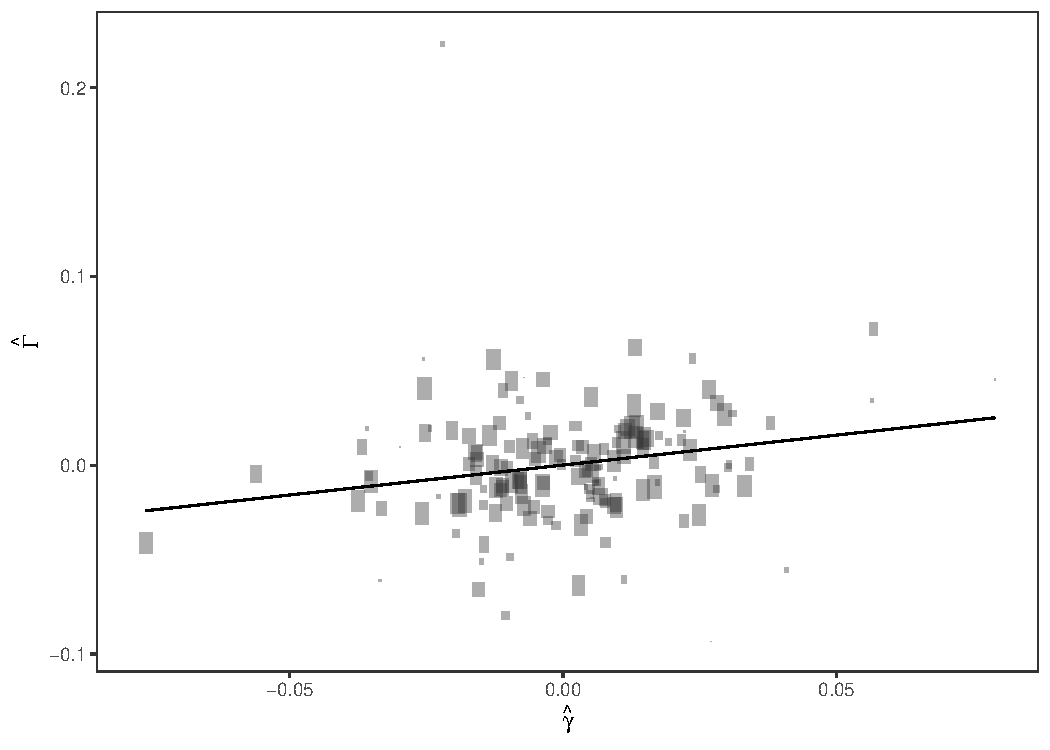
\includegraphics[width = \textwidth]{figures/MR_bmi_sdp.pdf}
\caption{按方差倒数加权的散点图及埃格回归线}\label{fig::bmi-sdp-egger}
\end{figure} 

 
\section{对孟德尔随机化分析法的若干批评}




孟德尔随机化是工具变量思想的具体应用，但其实施需满足诸多较强假设。下文从概念、生物学及技术三个层面对其进行评述。 



在概念层面，多数孟德尔随机化研究中的“处理因素”并未基于潜在结果框架予以清晰界定。例如，研究常将胆固醇水平或身体质量指数视为处理因素，然而它们均为复合变量，其对应的理想化实验定义方式亦不止一种；此时“无干扰无干扰无干扰无干扰”（SUTVA）假设往往难以满足。相关讨论可参见第\ref{chapter::potential-outcomes}章。 


从生物学角度而言，工具变量分析所需的基本前提可能并不成立。孟德尔第二定律虽保证了不同性状遗传的独立性，却未确保所选工具变量与处理因素和结局间的隐性混杂因素互不相关；事实上工具变量亦可能直接影响混杂因素，或某些未被测定的基因同时影响工具变量与混杂因素。此外，该定律亦无法保障排除性假设；工具变量还可能通过非处理因素作用路径影响结局。 


从技术上说，MR的统计假设相当强。线性工具变量模型显然是一个很强的建模假设。各$\hat\gamma_j$和各$\hat\Gamma_j$相互独立的假设也相当强。数据收集过程中的其他问题会进一步使工具变量假设的解释复杂化。例如，处理和结果通常带有测量误差，全基因组关联研究通常采用病例—对照设计，按结果进行抽样，见第\ref{sec::case-control}章。

 
\citet{vanderweele2014methodological}撰写了关于孟德尔随机化方法学挑战的优秀综述文献。 

 
 
\section{作业习题}

\paragraph{数据分析}\label{para::data-bmi-bmi}
分析\ri{R}包\ri{mr.raps}中的\ri{bmi.bmi}数据。更多细节见该包及\citet[][Section 7.2]{zhao2020statistical}。 


 
 \paragraph{推荐阅读}

\citet{davey2003mendelian}系统梳理了孟德尔随机化的优势及局限。 




